\chapter{Riemann-Stieltjes Integral}
\begin{define}[Partition]
	A partition $P$ of $[a,b]$ is $\{x_0,x_1,x_2,\ldots ,x_{n}\}$ for some $n\ge 1$, with $a=x_0\le x_1 \ldots \le x_{n-1}\le x_{n}=b$.\\
	\begin{notation}
		\begin{describe}
			\item[$\Delta x_i$]$=x_i-x_{i-1}$ for $i=1,\ldots ,n$
			\item[$f$]$: [a,b]\to \R$ be bounded, which is not necessarily continuous
			\item[$M_i$]$=\sup\{f(x):x_{i-1}\le x\le x_i\}$, $m_i=\inf\{f(x):x_{i-1}\le x\le x_i\}$
			\item[$U(P,f)$]$=\sum_{i=1}^{n}{M_i \Delta x_i}$
			\item[$L(P,f)$]$=\sum_{i=1}^{n}{m_{i}\Delta x_{i}}$.
		\end{describe}
	\end{notation}
	\begin{note}
		$L(P,f)\le U(p,f)$ always.
	\end{note}
\end{define}

\begin{define}[Riemann Integral]
	\begin{description}
		\item[Upper Riemann Integral]: $\overline{\int_{a}^{b}}f(x)dx=\inf_{P}\{ U(P,f)\}=\inf\{U(P,f):P\text{ is a partition of }[a,b]\}$.
		\item[Lower Riemann Integral]: $\underline{\int_{a}^{b}}f(x)dx=\sup_{P}\{L(P,f)\} =\sup\{L(P,f):P\text{ is a partition of }[a,b]\}$.
		\item[Riemann Integrable]: $f$ is Riemann integrable on $[a,b]$ if $\overline{\int_{a}^{b}}f(x)dx=\underline{\int_{a}^{b}}f(x)dx$.
		      If $f$ is Riemann integrable on $[a,b]$, we write $f \in \mathscr{R}[a,b]$ and
		      \[
			      \int_{a}^{b}f(x)dx=\overline{\int_{a}^{b}}f(x)dx=\underline{\int_{a}^{b}}f(x)dx.
		      \]

	\end{description}\hfill\\
	\begin{note}
		Since $f$ is bounded, $m=\inf\{f(x):a\le x\le b\}$ and $M=\sup\{f(x):a\le x\le b\}$ are both finite. Hence, for any $P$, $m\le m_i\le M_i\le M$ and $\forall_{i}: m(b-a)\le L(P,f)\le U(P,f)\le M(b-a)$.
	\end{note}
\end{define}
\hfill
\begin{notation}
	Let $\alpha:[a,b]\to \R$ is a monotone increasing function.
	Then $\Delta \alpha_i=\alpha(x_{i})-\alpha(x_{i-1})$.
\end{notation}

\begin{define}[2]
	Given $P$, let $\Delta \alpha_i=\alpha(x_{i})-\alpha(x_{i-1})$. (Note: $\Delta \alpha_i\ge 0$).\\
	For bounded $f$, let $U(P,f,\alpha)=\sum_{i=1}^{n}{M_{i} \Delta \alpha_i}$, $L(P,f,\alpha)=\sum_{i=1}^{n}{m_{i}}\Delta \alpha_i$.\\
	\begin{description}
		\item[Upper Riemann-Stieltjes Integral] $\overline{\int_{a}^{b}}f(x)d\alpha=\overline{\int_{a}^{b}}f(x)d\alpha(x)=\inf_{P}\{U(P,f,\alpha)\}=\inf\{U(P,f,\alpha):P\text{ is a partition of }[a,b]\}$.
		\item[Lower Riemann-Stieltjes Integral] $\underline{\int_{a}^{b}}f(x)d\alpha=\underline{\int_{a}^{b}}f(x)d\alpha(x)=\sup_{P}\{L(P,f,\alpha)\}=\sup\{L(P,f,\alpha):P\text{ is a partition of }[a,b]\}$.
	\end{description}\hfill\\
	If $\overline{\int_{a}^{b}}f(x)d\alpha=\underline{\int_{a}^{b}}f(x)d\alpha$, then $f\in R[a,b,\alpha]$ and $\int_{a}^{b}f(x)d\alpha=\overline{\int_{a}^{b}}f(x)d\alpha=\underline{\int_{a}^{b}}f(x)d\alpha$.\\
	If $\alpha(x)=x$, then equivalent to $\int_{a}^{b}f(x)dx$.
\end{define}

\begin{define}[3]
	\begin{enumerate}
		\item Partition $P^{*}$ is called a refinement of $P$ if $P\subset P^{*}$.
		\item Partition $P^{*}$ is called the common refinement of $P_1$ and $P_2$ if $P^{*}=P_1 \cup P_2$.
	\end{enumerate}
\end{define}

\begin{thm}[4]
	If $P^{*}$ is a refinement of $P$ then $L(P,f,\alpha)\le L(P^{*},f,\alpha)\le U(P^{*},f,\alpha)\le U(P,f,\alpha)$.
	\begin{proof}
		It's enough to consider $p^{*}$ with one extra point: $x_{i-1}\le x^{*}\le x_{i}$.\\
		Sketch for $L$:\\
		\begin{align*}
			 & L(P^{*},f,\alpha)-L(p,f,\alpha)                                                   \\
			 & = m^{*}[\alpha(x^{*})-\alpha(x_{i-1})]+m_i[\alpha(x_i)\alpha(x^{*})]
			-m_{i}[\alpha(x^{*})-\alpha(x_{i-1})]-m_i[\alpha(x_i)-\alpha(x^{*})]                 \\
			 & = (m^{*}-m_i)[\alpha(x^{*})-\alpha(x_{i-1})]+(m_i-m_i)[\alpha(x_i)-\alpha(x^{*})] \\
		\end{align*}
	\end{proof}
\end{thm}

\begin{notation}
	When $f,\alpha$ are fixed, we write $L(P)=L(P,f,\alpha),U(P)=U(P,f,\alpha)$
\end{notation}

\begin{thm}[5]
	$\underline{\int_{a}^{b}}{f\mathrm{d}\alpha}\le  \overline{\int_{a}^{b}}{f\mathrm{d}\alpha}$.
	\begin{proof}
		For partitions $P_1,P_2$, let $P^{*}=P_1 \cup P_2$.
		By Theorem~\ref{thm:6.4}, $L(P_1)\le L(P^{*})\le U(P^{*})\le U(P_2)$.
		In particular, $\sup_{P_1}\{L(P_1)\}\le U(P_2)$ for all $P_2$.
		Hence, $\sup_{P_1}\{L(P_1)\}\le \inf_{P_2}\{U(P_2)\}$.
	\end{proof}
\end{thm}
\begin{thm}[6]
	$f \in \mathscr{R}_{\alpha}[a,b]\Leftrightarrow \forall_{\epsilon > 0}: \exists P_{\epsilon} \text{ s.t. } U(P_{\epsilon})-L(P_{\epsilon})<\epsilon$
	\begin{proof}
		Let $\epsilon>0$.
		\begin{description}
			\item[$(\Rightarrow)$]
			      By hypothesis, $\sup_{P}\{L(P)\}= \underline{\int_{a}^{b}}f\mathrm{d}\alpha=\overline{\int_{a}^{b}}f\mathrm{d}\alpha=\inf_{P}\{U(P)\}$.\\
			      $\exists P_1,P_2$ s.t. $L(P_1)>\underline{\int_{a}^{b}}f\mathrm{d}\alpha-\epsilon/2$ and $U(P_2)<\overline{\int_{a}^{b}}f\mathrm{d}\alpha+\epsilon/2$.\\
			      Then $U(P_{2})-L(P_{1})<\epsilon$. Let $P_{\epsilon}=P^{*}=P_{1}\cup P_{2}$.
			      By Theorem~\ref{thm:6.4}, $L(P_{1})\le L(P^{*})\le U(P^{*})\le U(P_{2})$, so $U(P_{\epsilon})-L(P_{\epsilon})\le U(P_2)-L(P_1)<\epsilon$.
			\item[$(\Leftarrow)$]
			      $0\le \overline{\int_{a}^{b}}{f\mathrm{d}\alpha} - \underline{\int_{a}^{b}}{f\mathrm{d}\alpha}\le U(P_{\epsilon})-L(P_{\epsilon})<\epsilon$. Since $\epsilon$ is arbitrary, $\overline{\int_{a}^{b}}{f\mathrm{d}\alpha} = \underline{\int_{a}^{b}}{f\mathrm{d}\alpha}$.
		\end{description}
	\end{proof}
	\begin{remark}
		very important
	\end{remark}
\end{thm}

\begin{thm}[7]
	Let $\epsilon_0>0$ be fixed. Suppose there exists a partition $P=\{x_0=a,\ldots ,x_n=b\} $ s.t. $U(P,f,\alpha)-L(P,f,\alpha)<\epsilon_0$.
	Let $s_{i},t_{i}$ are arbitrary points in $[x_{i-1},x_i]$.
	Then,
	\begin{enumerate}
		\item For any refinement of $P$, denoted by $P^{*}$, $U(P^{*},f,\alpha)-L(P^{*},f,\alpha)<\epsilon_0$ also holds true
		\item  $\sum_{i=1}^{n}{\left|f(s_i)-f(t_i)\right| \Delta \alpha_i}<\epsilon_0$
		\item If $f \in \mathscr{R}_{\alpha}$, then $\left| \sum_{i=1}^{n}{f(t_i) \Delta \alpha_i}-\int_{a}^{b}{f\mathrm{d}\alpha} \right| <\epsilon_0$
	\end{enumerate}
\end{thm}


\begin{thm}[8]
	If $f$ is continuous on $[a,b]$ then $f \in \mathscr{R}_{\alpha}[a,b]$.
	\begin{proof}
		For any $P$, $U(P)-L(P)=\sum_{i=1}^{n}{(M_i - m_i) \Delta \alpha_i}$.
		Since $[a,b]$ is compact, $f$ is uniformly continuous on $[a,b]$ (Theorem~\ref{thm:4.19}), so $\forall{\eta > 0}: \exists{\delta > 0} \text{ s.t. } |x-t|<\delta \implies |f(x)-f(t)|<\eta$.
		Given $\epsilon > 0$, choose $\eta$ s.t. $\eta[\alpha(b)-\alpha(a)]<\epsilon$ and choose $P$ with $\Delta x_i<\delta=\delta(\eta)$ for all $i$.
		For such $P$, $M_i-m_i \le \eta$.
		Then $U(P)-L(P)\le \sum_{i=1}^{n}{\eta \Delta \alpha_i }=\eta[\alpha(b)-\alpha(a)]<\epsilon$.
		Therefore, $f \in \mathscr{R}_{\alpha}[a,b]$.
	\end{proof}
\end{thm}

\begin{thm}[9]
	If $f$ is monotone increasing or decreasing on $[a,b]$ and $\alpha$ is continuous on $[a,b]$ then $f \in \mathscr{R}_{\alpha}[a,b]$.
	\begin{proof}
		By definition, $U(P)-L(P)=\sum_{i=1}^{n}{(M_{i}-m_{i}) \Delta \alpha_i}$.
		Given $n \in \N$, let $P$ s.t. $\Delta \alpha_i = \dfrac{\alpha(b)-\alpha(a)}{n}$ for all $i$.
		Such $P$ exists by the intermediate value theorem (Theorem~\ref{thm:4.23}) as $\alpha$ is continuous.
		Then, $U(P)-L(P)=\dfrac{\alpha(b)-\alpha(a)}{n} \sum_{i=1}^{n}{M_{i}-m_{i}}$.
		Suppose $f$ is increasing, so $M_i - m_i=f(x_i)-f(x_{i-1})$.
		Then $U(P)-L(P)=\dfrac{\alpha(b)-\alpha(a)}{n}\sum_{i=1}^{n}{f(x_i)-f(x_{i-1})}=\dfrac{\alpha(b)-\alpha(a)}{n}[f(b)-f(a)]$.
		Given $\epsilon>0$, we can choose $n$ (hence $P$) s.t. $U(P)-L(P)<\epsilon$. Therefore, $f \in \mathscr{R}_{\alpha}[a,b]$ by Theorem~\ref{thm:6.6}.
	\end{proof}
	\begin{note}
		We always assume $\alpha$ is monotone.
	\end{note}
\end{thm}

\begin{thm}[10]
	If $f$ is bounded on $[a,b]$ and has only finitely many discontinuities, and $\alpha$ is continuous at each point where $f$ is not, then $f \in \mathscr{R}_{\alpha}[a,b]$.
	\begin{proof}
		We apply Theorem~\ref{thm:6.6}.
		Use $U(P)-L(P)=\sum_{i=1}^{n}{( M_{i}-m_{i} )\Delta \alpha_{i}}$.
		Let $\epsilon>0$ and $E=\{e_1,\ldots ,e_{k}\} $ be the set of points where $f$ is discontinuous.
		$\alpha$ is assumed to be continuous at each $e_i$, which implies $\exists{(u_j,v_j)} \text{ s.t. } u_j<e_j<v_j \text{ and } \alpha(v_j)-\alpha(u_j)<\epsilon$. (Relax inequality to include equality if $e_1=a$, $e_k=b$).\\
		Let $K=[a,b] \cap \left(\bigcup_{j=1}^{k}(u_j,v_j)\right)^{c}$. $K$ is compact.
		$f$ is continuous on $K$, so $f$ is uniformly continuous on $K$ by Theorem~\ref{thm:4.19}.
		Hence, $\exists{\delta>0} \text{ s.t. } \text{ for } s ,t \in K$, $|s-t|<\delta \implies |f(s)-f(t)|<\epsilon$.\\
		Form $P$ to consist of $\{u_1,v_1,\ldots ,u_{k},v_{k}\}$ and additional points in $K$ so that $\Delta x_i < \delta$.
		If $x_i$ is in $K$, then $M_i-m_i<\epsilon$.
		Otherwise, $x_i=u_j$ or $x_i=v_j$ for some $j$, so $\Delta \alpha_i \le \epsilon$. Then
		\begin{align*}
			0\le U(P)-L(P) & =\sum_{i=1}^{n}{(M_{i}-m_{i}) \Delta \alpha_i}                                                                                                                         \\
			               & \le \underbrace{k \cdot 2M \epsilon}_{\text{from intervals in $\bigcup_{j=1}^{k}(u_j,v_j)$}}+\underbrace{\epsilon[\alpha(b)-\alpha(a)]}_{\text{from intervals in $K$}}
			.
		\end{align*}
		As RHS is as small as we want by taking $\epsilon$ small enough, $f \in \mathscr{R}_{\alpha}[a,b]$.
	\end{proof}
	\begin{remark}
		\begin{enumerate}
			\item Theorem~\ref{thm:6.10} implies part of A1.2 but do the problem from first principles. Do not apply Theorem~\ref{thm:6.10} directly.
			\item A1.4 shows what can happen if $f,\alpha$ are discontinuous at the same point.
		\end{enumerate}
	\end{remark}
\end{thm}

\begin{thm}[11]
	If $f \in \mathscr{R}_{\alpha}[a,b], m \le f(x)\le M$ for all $x \in [a,b]$, and $\phi:[m,M]\to \R$ is continuous, then $\phi \circ f \in \mathscr{R}_{\alpha}[a,b]$.
	\begin{proof}
		Let $\epsilon>0$. As $\phi$ continuous on $[m,M]$, $\phi$ is uniformly continuous on $[m,M]$ by Theorem~\ref{thm:4.19}.
		That is, $\exists{\delta < \epsilon} \text{ s.t. } |\phi(s)-\phi(t)|<\epsilon$ if $|s-t|<\delta$ for $s,t \in [m,M]$.\\
		Since $f \in \mathscr{R}_{\alpha}$, there exists a partition $P=\{x_0,x_1,\ldots ,x_n\}$ of $[a,b]$ such that $U(P)-L(P)<\delta^2$.\\
		Let $A=\{i \in \{1,2,\ldots ,n\}: M_i -m_i < \delta\}, B=\{i \in \{1,2,\ldots ,n\}: M_i -m_i \ge  \delta\}$.
		Note $A \cup B=\{1,2,\ldots ,n\}$.
		\\
		Let $M^{*}_i=\sup\{\phi(f(x)):x_{i-1}\le x\le x_i\}$ and $m^{*}_i=\inf\{\phi(f(x)):x_{i-1}\le x\le x_i\}$.
		Suppose $i \in A$. Then $M_i-m_i<\delta$. By definition of $\delta$, this implies $|M^{*}_i-m^{*}_i|\le \epsilon$.\\
		Suppose $i \in B$.
		By definition of $P$,
		\[
			U(P,f,\alpha)-L(P,f,\alpha)=\sum_{i \in B}{(M_i-m_i)\Delta \alpha_i}<\delta ^2.
		\]
		As $M_i-m_i\ge \delta$,
		\[
			\delta \sum_{i \in B}{\Delta \alpha_i}\le \sum_{i \in B}{(M_i-m_i)\Delta \alpha_i}<\delta ^2
			.\]
		Hence, $\sum_{i \in B}{\Delta \alpha_i}<\delta$. Then,
		\begin{align*}
			 & \sum_{i \in B}{(M^{*}_i-m^{*}_i)\Delta \alpha_i}                                                                            \\
			 & \le 2 \cdot \underbrace{\sup\{|\phi|\}}_{=\sup\{|\phi(t)|: m\le t\le M\}} \cdot \left(\sum_{i \in B}{\Delta\alpha_i}\right) \\
			 & < 2\cdot \sup\{|\phi|\} \cdot \delta                                                                                        \\
			 & <2 \cdot \sup\{|\phi|\} \cdot \epsilon.
		\end{align*}
		Therefore,
		\begin{align*}
			 & U(P,\phi \circ f,\alpha)-L(P,\phi \circ f,\alpha)=\sum_{i=1}^{n}{(M^{*}_i-m^{*}_i)\Delta \alpha_i} \\
			 & =\sum_{i \in A}{(M^{*}_i-m^{*}_i)\Delta \alpha_i}+\sum_{i \in B}{(M^{*}_i-m^{*}_i)\Delta \alpha_i} \\
			 & < \epsilon[(\alpha(b)-\alpha(a)) + 2 \cdot \sup\{|\phi|\}]
		\end{align*}

	\end{proof}
	\begin{example}
		$f \in \mathscr{R}_{\alpha}[a,b]\implies f^2 \in \mathscr{R}_{\alpha}[a,b], |f| \in \mathscr{R}_{\alpha}[a,b]$ where $\phi(t)=t^2$ and $\phi(t)=|t|$ respectively.
	\end{example}
	\begin{note}
		$\phi \in \mathscr{R}_{\alpha}[m,M]$ does not imply $\phi \circ f \in \mathscr{R}_{\alpha}[a,b]$. See A2.
	\end{note}
\end{thm}

\begin{thm}[12](Linearity and related properties)
	\begin{enumerate}
		\item If $f,f_1,f_2 \in \mathscr{R}_{\alpha}[a,b]$, then $f_1+f_2 \in \mathscr{R}_{\alpha}[a,b]$, $cf \in \mathscr{R}_{\alpha}[a,b]$, and
		      \begin{align*}
			      \int_{a}^{b}{(f_1+f_2)\mathrm{d}\alpha} & =\int_{a}^{b}{f_1\mathrm{d}\alpha}+\int_{a}^{b}{f_2\mathrm{d}\alpha} \\
			      \int_{a}^{b}{c f\mathrm{d}\alpha}       & =c\int_{a}^{b}{f\mathrm{d}\alpha}.
		      \end{align*}
		      \begin{proof}
			      TEXTBOOK
		      \end{proof}
		\item $f_1,f_2 \in \mathscr{R}_{\alpha}$ and $f_1(x)\le f_2(x)$ for all $x \in [a,b]$, then $\int_{a}^{b}{f_1\mathrm{d}\alpha}\le \int_{a}^{b}{f_2\mathrm{d}\alpha}$.
		      \begin{proof}
			      $L(P,f_1)\le L(P,f_2)\le \sup_P L(P,f_2)=\int_{a}^{b}{f_2\mathrm{d}\alpha}$.
			      $\int_{a}^{b}{f_1\mathrm{d}\alpha}=\sup_{P}L(P,f_1)\le  \int_{a}^{b}{f_2\mathrm{d}\alpha}$.
		      \end{proof}
		\item If $f \in \mathscr{R}_{\alpha}[a,b], c \in [a,b]$ then $f \in \mathscr{R}_{\alpha}[a,c] \text{ and } f \in \mathscr{R}_{\alpha}[a,b] \text{ and }  \int_{a}^{b}{f\mathrm{d}\alpha}=\int_{a}^{c}{f\mathrm{d}\alpha}+\int_{c}^{b}{f\mathrm{d}\alpha}$.
		\item If $f \in \mathscr{R}_{\alpha} \text{ and }  |f(x)|\le M$ for all $x \in [a,b]$, then $|\int_{a}^{b}{f\mathrm{d}\alpha}|\le M(\alpha(b)-\alpha(a))$.
		      \begin{proof}
			      Let $P=\{a,b\}$. Then $-M[\alpha(b)-\alpha(a)]\le m_1 \Delta \alpha_1=L(P)\le \int_{a}^{b}{f\mathrm{d}\alpha}\le U(P)=M_1 \Delta \alpha_1\le M [\alpha(b)-\alpha(a)]$.
		      \end{proof}
		\item If $f \in \mathscr{R}_{\alpha_1} \text{ and }  f \in \mathscr{R}_{\alpha_2}$, then $f \in \mathscr{R}_{\alpha_1+\alpha_2}$ and
		      \begin{equation*}
			      \label{eq:s}
			      \int_{a}^{b}{f\mathrm{d}(\alpha_1+\alpha_2)}=\int_{a}^{b}{f\mathrm{d}\alpha_1}+\int_{a}^{b}{f\mathrm{d}\alpha_2} \tag{*}.
		      \end{equation*}\\
		      If $f \in \mathscr{R}_{\alpha} \text{ and }  c\ge 0$ then $f \in \mathscr{R}_{\alpha}$ and
		      $\int_{a}^{b}{f\mathrm{d}c \alpha}= c \int_{a}^{b}{f\mathrm{d}\alpha}$.
		      \begin{proof}[\ref{eq:s}]
			      Let $\epsilon>0$. Choose $P_1,P_2$ s.t. $U(P_{j},f,\alpha_j)-L(P_{j},f,\alpha_j)<\dfrac{\epsilon}{2}$, where $j=1,2$.
			      Let $P^{*}=P_1 \cup P_2$. By Theorem~\ref{thm:6.4},
			      \begin{equation*}
				      U(P^{*},f,\alpha_j)-L(P^{*},f,\alpha_j)<\dfrac{\epsilon}{2} \label{eq:ss}\tag{**}
				      .
			      \end{equation*}
			      Since $(\Delta \alpha_1)_i+(\Delta \alpha_2)_i=(\Delta(\alpha_1+\alpha_2))_i$,
			      \begin{align*}
				       & U(P^{*},f,(\alpha_1+\alpha_2))-L(P^{*},f,(\alpha_1+\alpha_2))                                                                     \\
				       & =\sum_{i=1}^{n}{(M_i-m_i)(\Delta(\alpha_1+\alpha_2))_i}                                                                           \\
				       & =\sum_{i=1}^{n}{(M_i-m_i)[(\Delta \alpha_1)_i+(\Delta \alpha_2)_i]}                                                               \\
				       & =\sum_{i=1}^{n}{(M_i-m_i)(\Delta \alpha_1)_i}+\sum_{i=1}^{n}{(M_i-m_i)(\Delta \alpha_2)_i}                                        \\
				       & =U(P^{*},f,\alpha_1)-L(P^{*},f,\alpha_1)+U(P^{*},f,\alpha_2)-L(P^{*},f,\alpha_2)<\dfrac{\epsilon}{2}+\dfrac{\epsilon}{2}=\epsilon
				      .\end{align*}
			      % adding gives $U(P^{*},f,\alpha_1+\alpha_2)-L(P^{*},f,\alpha_1+\alpha_2)<\dfrac{\epsilon}{2}+\dfrac{\epsilon}{2}=\epsilon$.
			      By Theorem~\ref{thm:6.6}, $f \in \mathscr{R}_{\alpha_1+\alpha_2}$.
			      Also $\int_{a}^{b}{f\mathrm{d}(\alpha_1+\alpha_2)}\le U(P^{*},f,\alpha_1+\alpha_2)=U(P^{*},f,\alpha_1)+U(P^{*},f,\alpha_2)<\int_{a}^{b}{f\mathrm{d}\alpha_1}+\dfrac{\epsilon}{2}+\int_{a}^{b}{f\mathrm{d}\alpha_2}+\dfrac{\epsilon}{2}$ by \eqref{eq:ss}.
			      Similarly, $\int_{a}^{b}{f\mathrm{d}(\alpha_1+\alpha_2)}\ge L(P^{*},f,\alpha_1+\alpha_2)=L(P^{*},f,\alpha_1)+L(P^{*},f,\alpha_2)>\int_{a}^{b}{f\mathrm{d}\alpha_1}-\dfrac{\epsilon}{2}+\int_{a}^{b}{f\mathrm{d}\alpha_2}-\dfrac{\epsilon}{2}$ by \eqref{eq:ss}. As $\epsilon$ is arbitrary, \eqref{eq:s} holds.
		      \end{proof}
	\end{enumerate}
\end{thm}
\begin{thm}[13]
	\begin{enumerate}
		\item $f,g \in \mathscr{R}_{\alpha}\implies fg \in \mathscr{R}_{\alpha}$
		      \begin{proof}
			      By Theorem~\ref{thm:6.11} with $\phi(t)=t^2$, $h \in \mathscr{R}_{\alpha}\implies h^2 \in \mathscr{R}_{\alpha}$.
			      By Theorem~\ref{thm:6.12}(a), $f,g \in \mathscr{R}_{\alpha}\implies f+g \in \mathscr{R}_{\alpha}$, so $(f\pm g)^2 \in \mathscr{R}_{\alpha}$.
			      % so $f^2 \in \mathscr{R}_{\alpha}$.
			      Since $(f+g)^2-(f-g)^2=4fg$, by Theorem~\ref{thm:6.12}(a), $fg \in \mathscr{R}_{\alpha}$.
		      \end{proof}
		\item If $f \in \mathscr{R}_{\alpha}$, then $|f| \in \mathscr{R}_{\alpha}$, and $\left|\int_{a}^{b}{f\mathrm{d}\alpha}\right|\le \int_{a}^{b}{|f|\mathrm{d}\alpha}$.
		      \begin{proof}
			      By Theorem~\ref{thm:6.11}, $|f| \in \mathscr{R}_{\alpha}$ (take $\phi(t)=|t|$).
			      Let \[
				      c=\sgn\left( \int_{a}^{b}{f\mathrm{d}\alpha}\right)=
				      \begin{cases}
					      +1 & \text{if } \int_{a}^{b}{f\mathrm{d}\alpha}>0 \\
					      0  & \text{if } \int_{a}^{b}{f\mathrm{d}\alpha}=0 \\
					      -1 & \text{if } \int_{a}^{b}{f\mathrm{d}\alpha}<0
				      \end{cases}
				      .\]
			      As $cf\le |f|$,
			      $\left|   \int_{a}^{b}{f\mathrm{d}\alpha}\right|=c\int_{a}^{b}{f\mathrm{d}\alpha}=\int_{a}^{b}{cf\mathrm{d}\alpha}\le \int_{a}^{b}{|f|\mathrm{d}\alpha}$.
		      \end{proof}
	\end{enumerate}

\end{thm}

\begin{define}[14][Unit Step Function]
	\label{def:unit_step}
	\[
		I(x)=\begin{cases}
			0 & x\le 0 \\
			1 & x>0
		\end{cases}
	\]
\end{define}

\begin{thm}[15]
	Suppose $f$ is bounded on $[a,b]$ and continuous at $s \in (a,b)$.
	Let \[
		\alpha(x)=\begin{cases}
			0 & x\le s \\
			1 & x>s
		\end{cases}
		.\]
	Then $\int_{a}^{b}{f\mathrm{d}\alpha}$ exists, and
	\[
		\int_{a}^{b}{f\mathrm{d}\alpha}=f (s).
	\]
	\begin{proof}
		Let $P=\{a,s,x,b\}$ with $x \in (s,b)$.
		$U(P)=\sum_{i=1}^{3}{M_i \Delta \alpha_i}=0+M_2 \Delta \alpha_1=M_2$.
		$L(P)=\sum_{i=1}^{3}{m_i \Delta \alpha_i}=0+m_2 \Delta \alpha_1=m_2$.
		Hence, $m_2 \le \underline{\int_{a}^{b}}{f\mathrm{d}\alpha}\le \overline{\int_{a}^{b}}{f\mathrm{d}\alpha}\le M_2$.
		Let $x$ approach $s$.
		By continuity of $f$ at $s$, $M_2$ approaches $f(s)$ from above and $m_2$ approaches $f(s)$ from below. Hence, $\underline{\int_{a}^{b}}{f\mathrm{d}\alpha}= f(s)= \overline{\int_{a}^{b}}{f\mathrm{d}\alpha}= \int_{a}^{b}{f\mathrm{d}\alpha}=f(s)$.\\
		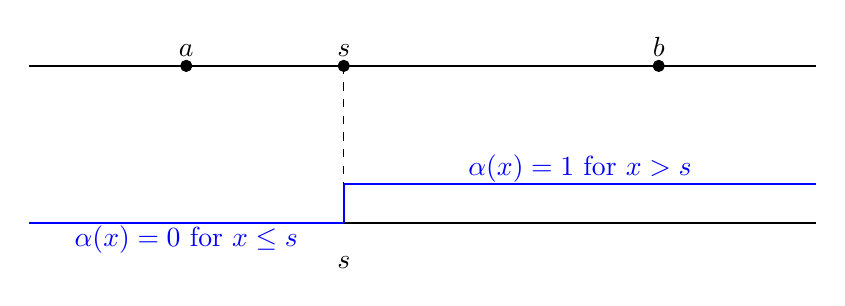
\begin{tikzpicture}
			\draw[thick] (0,0) -- (10,0);
			\filldraw (2,0) circle (2pt) node[above] {$a$};
			\filldraw (4,0) circle (2pt) node[above] {$s$};
			\filldraw (8,0) circle (2pt) node[above] {$b$};

			% Draw distances
			% \draw[<->] (2,0.5) -- (4,0.5) node[midway, above] {$|a-s|$};
			% \draw[<->] (4,0.5) -- (8,0.5) node[midway, above] {$|b-s|$};

			% Draw the alpha function line
			\draw[thick] (0,-2) -- (10,-2);
			\draw[dashed] (4,0) -- (4,-2);
			\node at (4,-2.5) {$s$};

			% Draw alpha function
			\draw[thick, blue] (0,-2) -- (4,-2);
			\draw[thick, blue] (4,-2) -- (4,-1.5);
			\draw[thick, blue] (4,-1.5) -- (10,-1.5);

			% Label alpha function
			\node[blue] at (2,-2.2) {$\alpha(x)=0$ for $x \leq s$};
			\node[blue] at (7,-1.3) {$\alpha(x)=1$ for $x > s$};
		\end{tikzpicture}
	\end{proof}
	\begin{remark}
		\begin{enumerate}
			\item By Theorem~\ref{thm:4.29}, if $\alpha$ is monotone-increasing,
			      then $\alpha(x^{+})$ and $\alpha(x^{-})$ exist for all $x \in (a,b)$, and $\alpha({x^{-}})\le \alpha(x)\le \alpha(x^{+})$.
			\item In Theorem~\ref{thm:6.15}, $\alpha$ is left-continuous at $s$.
			      \begin{exercise}
				      Prove the same conclusion for $\alpha(x)=\begin{cases}
						      0 & x<s    \\
						      1 & x\ge s
					      \end{cases}$.
			      \end{exercise}
			\item This $\alpha$ plays the role of the Dirac delta function:
			      \[
				      \int_{a}^{b}{f(x)\delta(x-s)dx}=f(s)
			      \]
			      where $\delta(x-s)=
				      \begin{cases}
					      0      & x\neq s \\
					      \infty & x=s
				      \end{cases}
			      $ is the Dirac delta function.
			      Technically, there is no such function as $\delta(x-s)$, but it is a useful concept in physics.
			      Note $\delta$ is kind of like $\alpha'$ in Theorem~\ref{thm:6.15}. (See A2).
			\item Theorem~\ref{thm:6.15} has $\alpha(x)=I(x-s)$.
		\end{enumerate}
	\end{remark}
\end{thm}

\begin{thm}[16]
	Let $c_{n}\ge 0, \sum_{n=1}^{\infty}{c_{n}}<\infty, s_{n} \in (a,b)$, where $s_i\neq s_j \text{ if } i\neq j$.\\
	Let $\alpha(x)=\sum_{n=1}^{\infty}{c_{n} I(x-s_{n})}$, a monotone increasing function.
	Let $f$ be continuous on $[a,b]$.
	Then $\int_{a}^{b}{f\mathrm{d}\alpha}=\sum_{n=1}^{\infty}{c_{n} f(s_{n})}$.
	\begin{note}
		\hfill
		\begin{enumerate}
			\item $\alpha(x)$ converges for any $x \in (a,b)$ by the comparison test, with
			      \begin{align*}
				      0\le \sum_{i=1}^{\infty}{c_{n} I(x-s_{n})}\le \sum_{n=1}^{\infty}{c_{n}}<\infty
			      \end{align*}
			\item $\sum_{n=1}^{\infty}{c_{n} f(s_{n})}$ converges by the comparison test, with
			      \begin{align*}
				      |c_{n} f(x_n)|\le M \cdot c_{n}
			      \end{align*}
		\end{enumerate}
	\end{note}

	\begin{proof}
		Let $R_N=\int_{a}^{b}{f\mathrm{d}\alpha}-\sum_{i=1}^{N}{c_{n}f(s_{n})}$.\\
		Claim: $R_N \to 0$ as $N \to \infty$; i.e., given $\epsilon>0$, $\exists{N_0} \text{ s.t. } |R_N|<\epsilon$ for all $N \ge N_0$.\\
		Let
		\begin{align*}
			\alpha_1(x) & =\sum_{n=1}^{N}{c_{n} I(x-s_{n})}         \\
			\alpha_2(x) & =\sum_{n=N+1}^{\infty}{c_{n} I(x-s_{n})}.
		\end{align*}
		By Theorem~\ref{thm:6.12} and Theorem~\ref{thm:6.15},
		\begin{align*}
			\int_{a}^{b}{f\mathrm{d}\alpha_1} & =\sum_{n=1}^{N}{c_{n} \int_{a}^{b}{f(x)\mathrm{d}I(x-s_{n})}}=\sum_{n=1}^{N}{c_{n} f(s_{n})} \\
			\int_{a}^{b}{f\mathrm{d}\alpha_2} & =\sum_{n=N+1}^{\infty}{c_{n} f(s_{n})}.
		\end{align*}
		By Theorem~\ref{thm:6.12},
		\begin{align*}
			\int_{a}^{b}{f\mathrm{d}\alpha}=\int_{a}^{b}{f\mathrm{d}\alpha_1}+\int_{a}^{b}{f\mathrm{d}\alpha_2}.
		\end{align*}
		Then $R_N=\int_{a}^{b}{f\mathrm{d}\alpha_2}$. Choose $N_0$ s.t. $\sum_{n=N_0+1}^{\infty}{c_{n}}<\epsilon$. By Theorem~\ref{thm:6.12}(d),
		\[
			|R_N|\le M\cdot [\alpha_2(b)-\underbrace{\alpha_2(a)}_{=0}]=M\cdot\sum_{n=N+1}^{\infty}{c_{n}}<M \cdot \epsilon
		\]
		for all $N \ge N_0$.
	\end{proof}
\end{thm}


\begin{thm}[17]
	Suppose
	\begin{enumerate}
		\item $|f(x)|\le M$ for all $x \in [a,b]$,
		\item $\alpha$ is differentiable on $[a,b]$ and increasing on $[a,b]$.
		\item $\alpha'(x) \in \mathscr{R}[a,b]$
	\end{enumerate}
	Then
	\begin{equation*}
		\label{eq:*}
		f \in \mathscr{R}_{\alpha}[a,b]\Leftrightarrow f \alpha' \in R[a,b] \tag{*}
	\end{equation*}
	If ~\eqref{eq:*} holds, then
	\begin{equation*}
		\label{eq:**}
		\int_{a}^{b}{f\mathrm{d}\alpha}=\int_{a}^{b}{f\alpha'\mathrm{d}x}\tag{**}
	\end{equation*}
	\begin{proof}
		\begin{enumerate}[label=(\roman*)]
			\item
			      It suffices to show that $\overline{\int_{a}^{b}}{f\mathrm{d}\alpha}=\overline{\int_{a}^{b}}{f\alpha'\mathrm{d}x}$ and $\underline{\int_{a}^{b}}{f\mathrm{d}\alpha}=\underline{\int_{a}^{b}}{f\alpha'\mathrm{d}x}$.
			\item
			      Let $\epsilon>0$. Since $\alpha' \in \mathscr{R}$, there exists $P$ s.t. $U(P,\alpha')-L(P,\alpha')<\epsilon$ by Theorem~\ref{thm:6.6}.\\
			      Note this and the rest of the proof hold for any refinement of $P$.
			      $U(P,\alpha')-L(P,\alpha')=\sum_{i=1}^{n}{(A_i-a_i)}\Delta x_i$,
			      where $A_i=\sup\{\alpha'(x):x \in [x_{i-1},x_i]\}$ and $a_i=\inf\{\alpha'(x):x_{i-1}\le x\le x_i\}$.
			      By \hyperref[thm:mean-value-theorem]{the mean value theorem},
			      \[
				      \exists{t_1 \in [x_{i-1},x_{i}]} \text{ s.t. } \Delta \alpha_i=\alpha'(t_i) \cdot \Delta x_{i}
				      .\]
			      For any $s_i \in [x_{i-1},x_i]$, $\left|  \alpha'(s_i)-\alpha'(t_i)\right|\le A_{i}-a_{i}$, so
			      \[
				      \sum_{i=1}^{n}{\left|\alpha'(s_{i})-\alpha'(t_{i})\right| \Delta x_{i}}<\epsilon
				      .\]
			      [cf. Theorem~\ref{thm:6.7}(b)]
			\item
			      For any $s_i \in [x_{i-1},x_i]$,
			      \[
				      \left|\sum_{i=1}^{n}{f(s_{i})\cdot  \underbrace{\Delta \alpha_i}_{\alpha'(t_i) \Delta x_i}} - \sum_{i=1}^{n}{f(s_i)\alpha'(s_{i}) \Delta x_{i}}\right|
				      =\left|\sum_{i=1}^{n}{f(s_i)[\alpha'(t_i)-\alpha'(s_i)]\Delta x_i}\right|<M \epsilon
				      .\]
			      Therefore,
			      \[
				      \sum_{i=1}^{n}{f(s_i)\Delta \alpha_i}\le \sum_{i=1}^{n}{f(s_i)\alpha'(s_i)\Delta x_i+M\epsilon}\le U(P,f\alpha')+M \epsilon
				      .\]
			      Taking supremum over $s_i$'s, $U(P,f,\alpha)\le U(P,f\alpha')+M \epsilon$, so
			      \begin{align*}
				      \overline{\int_{a}^{b}}{f\mathrm{d}\alpha} & \le U(P,f,\alpha)             \\
				                                                 & \le U(P,f\alpha')+M \epsilon.
			      \end{align*}
			      As $\inf_{P}U(P,f,\alpha)\le \inf_{P}U(P,f\alpha')$,
			      \[
				      \overline{\int_{a}^{b}}{f\mathrm{d}\alpha}\le \overline{\int_{a}^{b}}{f \alpha'\mathrm{d}x} +M \epsilon
				      .\]
			      Since $\epsilon>0$ is arbitrary,
			      \[
				      \overline{\int_{a}^{b}}{f\mathrm{d}\alpha}\le \overline{\int_{a}^{b}}{f\alpha'\mathrm{d}x}
				      .\]
			      Similarly, $\underline{\int_{a}^{b}}{f\mathrm{d}\alpha}\ge \underline{\int_{a}^{b}}{f\alpha'\mathrm{d}x}$.
		\end{enumerate}
	\end{proof}
\end{thm}

\begin{thm}[19][Change of Variables]\label{thm:change_of_variables}\\
	Suppose $\phi:[A,B]\to [a,b]$ is strictly increasing, continuous, and onto.
	Suppose $\alpha$ is increasing on $[a,b]$ and $f \in \mathscr{R}_{\alpha}[a,b]$.
	Let $g=f \circ \phi: [A,B]\to \R, \beta=\alpha \circ \phi: [A,B]\to \R$.
	Then $g \in \mathscr{R}_{\beta}[A,B] \text{ and } \int_{A}^{B}{g\mathrm{d}\beta}= \int_{a}^{b}{f\mathrm{d}\alpha}$.
	\begin{note}
		This is the change of variables formula for Riemann-Stieltjes integrals.
		It generalizes the calculus formula.
		$\int_{a}^{b}{f(x)\mathrm{d}x}=\int_{{\phi ^{-1}}(a)}^{\phi^{-1}(b)}{f(\phi(y))\phi'(y)\mathrm{d}y}$. Here $\alpha(x)=x$, so $\beta=\phi$ and $\mathrm{d}\beta=\phi'(y)\mathrm{d}y$
	\end{note}

	\begin{proof}
		Partition $P$ of $[a,b]$ and $Q$ of $[A,B]$ are in one-to-one correspondence via $x_i=\phi(y_i)$.
		$g([y_{i-1},y_{i}])=f([x_{i-1},x_{i}])$ and $\alpha(x_{i})=(\alpha \circ \phi)(y_i)=\beta(y_i)$, so $U(P,f,\alpha)=U(Q,g,\beta)$, and $L(P,f,\alpha)=L(Q,g,\beta)$.
		Let $\epsilon>0$. Since $f \in \mathscr{R}_{\alpha}[a,b]$, there exists $P$ s.t. $U(P,f,\alpha)-L(P,f,\alpha)<\epsilon$, so $U(Q,g,\beta)-L(Q,g,\beta)<\epsilon$, and $g \in \mathscr{R}_{\beta}[A,B]$.
		Also, $\int_{A}^{B}{g\mathrm{d}\beta}=\inf_{Q}U(Q,g,\beta)=\inf_{P}(P,f,\alpha)=\int_{a}^{b}{f\mathrm{d}\alpha}$.
	\end{proof}
	\begin{example}
		$\int_{a}^{b}{\sin{x^2}\mathrm{d}x}$ for $0\le a<b$.
		Here, $f(x)=\sin{x^2},\alpha(x)=x$.
		Let $x^2=y$, so $x=\phi(y)=\sqrt[]{y}, \phi^{-1}(y)=y^2$.
		Then $\phi:\underbrace{[a^2,b^2]}_{=[A,B]}\to [a,b]$ is continuous, strictly increasing, and onto.
		$g(y)=(f \circ \phi)(y)=\sin{y}$.
		$\beta(y)=(\alpha \circ \phi)(y)=\sqrt[]{y}$.
		Theorem~\ref{thm:6.19} gives
		\[
			\int_{a}^{b}{\sin{x^2}\mathrm{d}dx}
			=\int_{a^2}^{b^2}{\sin{y}\mathrm{d}\beta}
			=\int_{a^2}^{b^2}{\sin{y}\dfrac{1}{2\sqrt[]{y}}\mathrm{d}y}
			,\]
		where the last equality follows from the Theorem~\ref{thm:6.17} as $\beta'=\dfrac{1}{2 \sqrt[]{y}} \in \mathscr{R}[a^2,b^2]$.
		Hence,
		\[
			\int_{a}^{b}{\sin{x^2}\mathrm{d}x}=\int_{a^2}^{b^2}{\dfrac{\sin{y}}{2\sqrt[]{y}}\mathrm{d}y}.
		\]
	\end{example}
\end{thm}

\begin{thm}[20]
	Let $f \in \mathscr{R}[a,b]$ and for $x \in [a,b]$, define $F(x)= \int_{a}^{x}{f(t)\mathrm{d}t}$. Then $F$ is continuous on $[a,b]$, and if $f$ is continuous at $x_0 \in [a,b]$, then $F'(x_0)$ exists and $F'(x_0)=f(x_0)$.\\
	\begin{proof}
		\begin{description}
			\item[Continuity of $F$]:
			      Choose $M$ s.t. $\left|f(t)\right|\le M$ for all $t \in [a,b]$.
			      For $a\le x<y\le b$, $\left|F(y)-F(x)\right|=\left|\int_{a}^{y}{f(t)\mathrm{d}t}- \int_{a}^{x}{f(t)\mathrm{d}t}\right|= \left|\int_{x}^{y}{f(t)\mathrm{d}t}\right|\le M \left|y-x\right|$.
			      Let $\epsilon>0$. If $\left|y-x\right|<\delta=\dfrac{\epsilon}{M}$, then $\left|F(y)-F(x)\right|<M\cdot \dfrac{\epsilon}{M} = \epsilon$. Therefore, $F$ is continuous on $[a,b]$.
			\item[Differentiability of $F$ and $F'(x_0)=f(x_0)$]: Let $h>0$.
			      \[
				      \dfrac{[F(x_0+h)-F(x_0)}{h}-f(x_0)=\dfrac{1}{h}\left[\int_{x_0}^{x_0+h}{f(t)\mathrm{d}t}\right]-f(x_0)=\dfrac{1}{h} \int_{x_0}^{x_0+h}{[f(t)-f(x_0)]\mathrm{d}t}
				      .\]
			      As $f$ is continuous at $x_0$, $\forall{\epsilon > 0}: \exists{\delta > 0} \text{ s.t. } \left|t-x_0\right|< \delta \implies \left|f(t)-f(x_0)\right| < \epsilon$. Thus, if $h<\delta$,
			      \[
				      \left|\dfrac{[F(x_0+h)-F(x_0)}{h}-f(x_0)\right|= \left|\dfrac{1}{h} \int_{x_0}^{x_0+h}{\underbrace{\left[f(t)-f(x_0)\right] }_{ \in (-\epsilon,\epsilon)}\mathrm{d}t}\right|\le \dfrac{1}{h} \cdot h \epsilon=\epsilon
			      \]
		\end{description}
	\end{proof}
\end{thm}

\begin{thm}[21][Fundamental Theorem of Calculus]
	\label{thm:ftc}
	If $f \in \mathscr{R}[a,b]$ and if $\exists$ differentiable function $F$ on $[a,b]$ s.t. $F'=f$, then $\int_{a}^{b}{f(x)\mathrm{d}x}=F(b)-F(a)$.
	\begin{proof}
		For any partition $P$, $F(b)-F(a)=\sum_{i=1}^{n}{[F(x_{i})-F(x_{i-1})]}$, and by the mean value theorem~\ref{thm:mvt},
		\[
			\forall{i \in \{1,2,\ldots ,n\} }:\exists{t_i \in [x_{i-1},x_{i}]} \text{ s.t. } F(x_{i})-F(x_{i-1})=F'(t_i) \Delta x_i=f(t_i) \Delta x_i
			.\]
		Therefore,
		\[
			F(b)-F(a)=\sum_{i=1}^{n}{F'(t_i) \Delta x_i}=\left[\sum_{i=1}^{n}{\underbrace{f(t_i)}_{\in [m_i,M_i]} \Delta x_i}\right] \in [L(P,f),U(P,f)]
			.\]
		% \[
		% 	\exists{t_i \in [x_{i-1},x_{i}]} \text{ s.t. } \sum_{i=1}^{n}{F'(t_i)} \Delta x_i=\sum_{i=1}^{n}{\underbrace{f(t_i)}_{\in [m_i,M_i]}}\Delta x_i \in [L(P,f),U(P,f)]
		% 	.\]
		Also, $\int_{a}^{b}{f(t)\mathrm{d}t} \in [L(P,f),U(P,f)]$.\\
		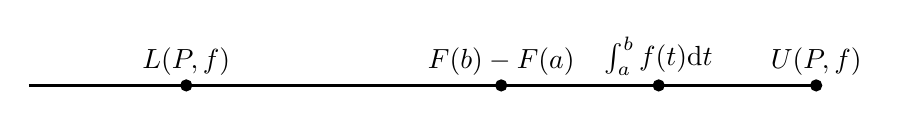
\begin{tikzpicture}
			\draw[thick] (0,0) -- (10,0);
			\filldraw (2,0) circle (2pt) node[above] {$L(P,f)$};
			\filldraw (6,0) circle (2pt) node[above] {$F(b)-F(a)$};
			\filldraw (8,0) circle (2pt) node[above] {$\int_{a}^{b}{f(t)\mathrm{d}t}$};
			\filldraw (10,0) circle (2pt) node[above] {$U(P,f)$};
		\end{tikzpicture}\\
		Let $\epsilon>0$. Choose $P$ s.t. $U(P,f)-L(P,f)<\epsilon$. Then
		\[
			\left|[F(b)-F(a)]-\int_{a}^{b}{f(t)\mathrm{d}t}\right|<\epsilon
			.\]
		Since $\epsilon>0$ is arbitrary, $\left|[F(b)-F(a)]-\int_{a}^{b}{f(t)\mathrm{d}t}\right|=0$.
	\end{proof}
\end{thm}

\begin{thm}[22][Integration by Parts]
	\label{thm:ibp}
	If $F,G$ are differentiable on $[a,b]$ and $F'=f,G'=g \in \mathscr{R}[a,b]$, then
	\begin{equation*}
		\int_{a}^{b}{F(x)g(x)\mathrm{d}x}=F(b)G(b)-F(a)G(a)-\int_{a}^{b}{f(x)G(x)\mathrm{d}x}\\
		.\end{equation*}
	Moreover, if $F,G$ are (monotone) increasing, on $[a,b]$, then
	\begin{equation*}
		\int_{a}^{b}{F\mathrm{d}G}=FG|_{a}^{b}-\int_{a}^{b}{G\mathrm{d}F}
		.\end{equation*}
	\begin{proof}
		Let $H(x)=F(x)G(x)$.
		Then $H'=F'G+FG'=fG + Fg \in \mathscr{R}[a,b]$, so
		\[
			\int_{a}^{b}{H'(x)\mathrm{d}x} =\int_{a}^{b}{f(x)G(x)\mathrm{d}x}+\int_{a}^{b}{F(x)g(x)\mathrm{d}x}
			.\]
		By Theorem~\ref{thm:ftc} to $H$,
		\begin{align*}
			\int_{a}^{b}{H'(x)\mathrm{d}x}               & =H(b)-H(a)=F(b)G(b)-F(a)G(a)                                         \\
			                                             & =\int_{a}^{b}{f(x)G(x)\mathrm{d}x}+\int_{a}^{b}{F(x)g(x)\mathrm{d}x} \\
			\therefore \int_{a}^{b}{F(x)g(x)\mathrm{d}x} & =F(b)G(b)-F(a)G(a)-\int_{a}^{b}{f(x)G(x)\mathrm{d}x}
			.\end{align*}
	\end{proof}

	\begin{remark}
		See problem 6.17 for a version with $\alpha$.
	\end{remark}
\end{thm}

\begin{define}[Limits of Integration]
	If $f \in \mathscr{R}[a,b]$ for all $b>0$, then we define $\int_{a}^{\infty}{f(x)\mathrm{d}x}=\lim_{b\to \infty}{\int_{a}^{b}{f(x)\mathrm{d}x}}$ if the limit exists (in $(-\infty,\infty)$) and we say $\int_{a}^{\infty}{f(x)\mathrm{d}x}$ converges.
	If $\int_{a}^{\infty}{\left|f(x)\right|\mathrm{d}x}$ converges, then we say the integral converges absolutely.
\end{define}

\begin{example}[1]
	Prove that $\int_{0}^{\infty}{\sin{t^2}\mathrm{d}t}$ converges but not absolutely.
	[$\int_{0}^{x}{\sin{t^2}\mathrm{d}t}$ is a Fresnel integral and $\int_{0}^{\infty}{\sin{t^2}\mathrm{d}t}= \sqrt{\dfrac{\pi}{8}}$, as can be shown by contour integration.]
	\begin{proof}
		Let $I_x=\int_{0}^{x}{\sin{t^2}\mathrm{d}t}$ for $x>0$.
		\begin{description}
			\item[Proof of Convergence]:
			      \begin{enumerate}
				      \item
				            Claim: $I_n$ is a Cauchy Sequence $(n \in \N)$, so it has a limit in $\R$.
				            \begin{proof}
					            For $0<x<y$, $\int_{x}^{y}{\sin{t^2}\mathrm{d}t}=\int_{x^2}^{y^2}{\sin{u} \cdot \dfrac{1}{2 \sqrt{u}}\mathrm{d}u}$.
					            Using Theorem~\ref{thm:ibp},
					            \begin{align*}
						            \int_{x^2}^{y^2}{\underbrace{\dfrac{1}{2 \sqrt{u}}}_{F(u)}\cdot  \underbrace{\vphantom{\dfrac{1}{2 \sqrt{u}}}\sin{u}\mathrm{d}u}_{\mathclap{\mathrm{d}G(u)}}} & =FG \bigg\rvert_{x^2}^{y^2}- \int_{x^2}^{y^2}{G\mathrm{d}F}                                                                                                           \\
						                                                                                                                                                                          & =\dfrac{\cos{y^2}}{2y}+\dfrac{\cos{x^2}}{2x}-\int_{x^2}^{y^2}{\cos{u}\dfrac{1}{4u^{3/2}}\mathrm{d}u}                                                                  \\
						            \therefore \left|I_x-I_y\right|                                                                                                                               & \le \frac{1}{2y}+\frac{1}{2x}+\underbrace{\int_{x^2}^{y^2}{\frac{1}{4u^{3/2}}\mathrm{d}u}}_{\left.-\frac{1}{2u^{1/2}} \right|_{x^2}^{y^2}=-\frac{1}{2y}+\frac{1}{2x}} \\
						                                                                                                                                                                          & =\dfrac{1}{x}
						            .\end{align*}
					            In particular, for $n\ge m$, $\left|I_n-I_m\right|\le \dfrac{1}{m}$, so $(I_n)$ is a Cauchy sequence.
					            Therefore, $\exists{ I \in \R} \text{ s.t. } I_n\to I$ as $n\to \infty$.
				            \end{proof}

				      \item Let $\epsilon>0$. Choose $N_0>\dfrac{1}{\epsilon}$, so that $N\ge N_0\implies \left|I_N-I\right|<\epsilon$.
				            Let $b> N_0$. Choose $N$ s.t. $b \in [N,N+1)$.
				            As $N_0 \le N$
				            \[
					            I_b=\int_{0}^{b}{\sin{t^2}\mathrm{d}t}=I_N+ \int_{N}^{b}{\sin{t^2}\mathrm{d}t}\le I_N+\dfrac{1}{N}
					            .\]
				            Hence, \[
					            \left|I-I_b\right| \le \left|I-I_N\right|+\dfrac{1}{N} <\dfrac{1}{N}+\dfrac{1}{N}= \dfrac{2}{N}\le \dfrac{2}{N_0} <2 \epsilon
					            .\]
				            \[
					            \therefore \int_{0}^{\infty}{\sin{t^2}\mathrm{d}t}=I
					            .\]
			      \end{enumerate}
			\item[Failure of Absolute Convergence]:
			      \begin{proof}
				      For $n\ge 0$, let $[A_n,B_{n}]=[2n\pi,(2n+1)\pi]$, and let $a_n^2=A_n,b_{n}^{2}=B_n$.\\
				      Then $\int_{0}^{b_N}{\left|\sin{t^2}\right|\mathrm{d}t}\ge \sum_{n=0}^{N}{\int_{a_n}^{b_n}{\sin{t^2}\mathrm{d}t}}$.
				      Now
				      \[
					      \int_{a_n}^{b_n}{\sin{t^2}\mathrm{d}t}=\int_{A_n}^{B_n}{\sin{u}\cdot \dfrac{1}{2 \sqrt{u}}\mathrm{d}u}\ge \dfrac{1}{2 \sqrt{B_n}} \cdot  \int_{A_n}^{B_n}{\sin{u}\mathrm{d}u}=\dfrac{1}{\sqrt{B_n}}
					      .\]
				      \[
					      \therefore \int_{0}^{b_N}{\left|\sin{t^2}\right|\mathrm{d}t}\ge \sum_{n=0}^{N}{\frac{1}{\sqrt{(2n+1)\pi}}}= \frac{1}{\sqrt{\pi}}\cdot  \underbrace{\sum_{n=0}^{N}{\frac{1}{\sqrt{2n+1}}}}_{\to \infty \text{ as } N\to \infty}
					      .\]
				      Hence,
				      \[
					      \int_{0}^{\infty}{\left|\sin{t^2}\right|\mathrm{d}t}=\infty
					      .\]
			      \end{proof}
		\end{description}
	\end{proof}
\end{example}

\begin{note}
	Material for MT 1 ends here, including A1,A2,A3.
\end{note}
